
%% bare_conf.tex
%% V1.3
%% 2007/01/11
%% by Michael Shell
%% See:
%% http://www.michaelshell.org/
%% for current contact information.
%%
%% This is a skeleton file demonstrating the use of IEEEtran.cls
%% (requires IEEEtran.cls version 1.7 or later) with an IEEE conference paper.
%%
%% Support sites:
%% http://www.michaelshell.org/tex/ieeetran/
%% http://www.ctan.org/tex-archive/macros/latex/contrib/IEEEtran/
%% and
%% http://www.ieee.org/

%%*************************************************************************
%% Legal Notice:
%% This code is offered as-is without any warranty either expressed or
%% implied; without even the implied warranty of MERCHANTABILITY or
%% FITNESS FOR A PARTICULAR PURPOSE! 
%% User assumes all risk.
%% In no event shall IEEE or any contributor to this code be liable for
%% any damages or losses, including, but not limited to, incidental,
%% consequential, or any other damages, resulting from the use or misuse
%% of any information contained here.
%%
%% All comments are the opinions of their respective authors and are not
%% necessarily endorsed by the IEEE.
%%
%% This work is distributed under the LaTeX Project Public License (LPPL)
%% ( http://www.latex-project.org/ ) version 1.3, and may be freely used,
%% distributed and modified. A copy of the LPPL, version 1.3, is included
%% in the base LaTeX documentation of all distributions of LaTeX released
%% 2003/12/01 or later.
%% Retain all contribution notices and credits.
%% ** Modified files should be clearly indicated as such, including  **
%% ** renaming them and changing author support contact information. **
%%
%% File list of work: IEEEtran.cls, IEEEtran_HOWTO.pdf, bare_adv.tex,
%%                    bare_conf.tex, bare_jrnl.tex, bare_jrnl_compsoc.tex
%%*************************************************************************

% *** Authors should verify (and, if needed, correct) their LaTeX system  ***
% *** with the testflow diagnostic prior to trusting their LaTeX platform ***
% *** with production work. IEEE's font choices can trigger bugs that do  ***
% *** not appear when using other class files.                            ***
% The testflow support page is at:
% http://www.michaelshell.org/tex/testflow/



% Note that the a4paper option is mainly intended so that authors in
% countries using A4 can easily print to A4 and see how their papers will
% look in print - the typesetting of the document will not typically be
% affected with changes in paper size (but the bottom and side margins will).
% Use the testflow package mentioned above to verify correct handling of
% both paper sizes by the user's LaTeX system.
%
% Also note that the "draftcls" or "draftclsnofoot", not "draft", option
% should be used if it is desired that the figures are to be displayed in
% draft mode.
%
\documentclass[10pt, conference, compsocconf]{IEEEtran}
% Add the compsocconf option for Computer Society conferences.
%
% If IEEEtran.cls has not been installed into the LaTeX system files,
% manually specify the path to it like:
% \documentclass[conference]{../sty/IEEEtran}





% Some very useful LaTeX packages include:
% (uncomment the ones you want to load)


% *** MISC UTILITY PACKAGES ***
%
%\usepackage{ifpdf}
% Heiko Oberdiek's ifpdf.sty is very useful if you need conditional
% compilation based on whether the output is pdf or dvi.
% usage:
% \ifpdf
%   % pdf code
% \else
%   % dvi code
% \fi
% The latest version of ifpdf.sty can be obtained from:
% http://www.ctan.org/tex-archive/macros/latex/contrib/oberdiek/
% Also, note that IEEEtran.cls V1.7 and later provides a builtin
% \ifCLASSINFOpdf conditional that works the same way.
% When switching from latex to pdflatex and vice-versa, the compiler may
% have to be run twice to clear warning/error messages.






% *** CITATION PACKAGES ***
%
%\usepackage{cite}
% cite.sty was written by Donald Arseneau
% V1.6 and later of IEEEtran pre-defines the format of the cite.sty package
% \cite{} output to follow that of IEEE. Loading the cite package will
% result in citation numbers being automatically sorted and properly
% "compressed/ranged". e.g., [1], [9], [2], [7], [5], [6] without using
% cite.sty will become [1], [2], [5]--[7], [9] using cite.sty. cite.sty's
% \cite will automatically add leading space, if needed. Use cite.sty's
% noadjust option (cite.sty V3.8 and later) if you want to turn this off.
% cite.sty is already installed on most LaTeX systems. Be sure and use
% version 4.0 (2003-05-27) and later if using hyperref.sty. cite.sty does
% not currently provide for hyperlinked citations.
% The latest version can be obtained at:
% http://www.ctan.org/tex-archive/macros/latex/contrib/cite/
% The documentation is contained in the cite.sty file itself.






% *** GRAPHICS RELATED PACKAGES ***
%
\ifCLASSINFOpdf
  % \usepackage[pdftex]{graphicx}
  % declare the path(s) where your graphic files are
  % \graphicspath{{../pdf/}{../jpeg/}}
  % and their extensions so you won't have to specify these with
  % every instance of \includegraphics
  % \DeclareGraphicsExtensions{.pdf,.jpeg,.png}
\else
  % or other class option (dvipsone, dvipdf, if not using dvips). graphicx
  % will default to the driver specified in the system graphics.cfg if no
  % driver is specified.
  % \usepackage[dvips]{graphicx}
  % declare the path(s) where your graphic files are
  % \graphicspath{{../eps/}}
  % and their extensions so you won't have to specify these with
  % every instance of \includegraphics
  % \DeclareGraphicsExtensions{.eps}
\fi
% graphicx was written by David Carlisle and Sebastian Rahtz. It is
% required if you want graphics, photos, etc. graphicx.sty is already
% installed on most LaTeX systems. The latest version and documentation can
% be obtained at: 
% http://www.ctan.org/tex-archive/macros/latex/required/graphics/
% Another good source of documentation is "Using Imported Graphics in
% LaTeX2e" by Keith Reckdahl which can be found as epslatex.ps or
% epslatex.pdf at: http://www.ctan.org/tex-archive/info/
%
% latex, and pdflatex in dvi mode, support graphics in encapsulated
% postscript (.eps) format. pdflatex in pdf mode supports graphics
% in .pdf, .jpeg, .png and .mps (metapost) formats. Users should ensure
% that all non-photo figures use a vector format (.eps, .pdf, .mps) and
% not a bitmapped formats (.jpeg, .png). IEEE frowns on bitmapped formats
% which can result in "jaggedy"/blurry rendering of lines and letters as
% well as large increases in file sizes.
%
% You can find documentation about the pdfTeX application at:
% http://www.tug.org/applications/pdftex





% *** MATH PACKAGES ***
%
%\usepackage[cmex10]{amsmath}
% A popular package from the American Mathematical Society that provides
% many useful and powerful commands for dealing with mathematics. If using
% it, be sure to load this package with the cmex10 option to ensure that
% only type 1 fonts will utilized at all point sizes. Without this option,
% it is possible that some math symbols, particularly those within
% footnotes, will be rendered in bitmap form which will result in a
% document that can not be IEEE Xplore compliant!
%
% Also, note that the amsmath package sets \interdisplaylinepenalty to 10000
% thus preventing page breaks from occurring within multiline equations. Use:
%\interdisplaylinepenalty=2500
% after loading amsmath to restore such page breaks as IEEEtran.cls normally
% does. amsmath.sty is already installed on most LaTeX systems. The latest
% version and documentation can be obtained at:
% http://www.ctan.org/tex-archive/macros/latex/required/amslatex/math/





% *** SPECIALIZED LIST PACKAGES ***
%
%\usepackage{algorithmic}
% algorithmic.sty was written by Peter Williams and Rogerio Brito.
% This package provides an algorithmic environment fo describing algorithms.
% You can use the algorithmic environment in-text or within a figure
% environment to provide for a floating algorithm. Do NOT use the algorithm
% floating environment provided by algorithm.sty (by the same authors) or
% algorithm2e.sty (by Christophe Fiorio) as IEEE does not use dedicated
% algorithm float types and packages that provide these will not provide
% correct IEEE style captions. The latest version and documentation of
% algorithmic.sty can be obtained at:
% http://www.ctan.org/tex-archive/macros/latex/contrib/algorithms/
% There is also a support site at:
% http://algorithms.berlios.de/index.html
% Also of interest may be the (relatively newer and more customizable)
% algorithmicx.sty package by Szasz Janos:
% http://www.ctan.org/tex-archive/macros/latex/contrib/algorithmicx/






% correct bad hyphenation here
\hyphenation{op-tical net-works semi-conduc-tor}
\usepackage{multirow}
\usepackage{amsmath}
\usepackage{systeme}
\usepackage{graphicx}
\usepackage{subcaption}
\usepackage{caption}

\begin{document}
%
% paper title
% can use linebreaks \\ within to get better formatting as desired
%\title{Quantification of energy savings in smart buildings, physics or data?}

%\title{A novel data driven approach for the quantification of energy savings in smart buildings}
\title{Data driven modeling for energy consumption prediction in smart buildings}
 
 
% author names and affiliations
% use a multiple column layout for up to two different
% affiliations

\author{\IEEEauthorblockN{Aurora Gonz\'alez-Vidal}
\IEEEauthorblockA{Department of Information and Communication Engineering\\
Computer Science\\
University of Murcia, Spain\\
aurora.gonzalez2@um.es}
\and
\IEEEauthorblockN{Alfonso P. Ramallo-Gonz\'alez}
\IEEEauthorblockA{Department of Information and Communication Engineering\\
Computer Science\\
University of Murcia, Spain\\
alfonsop.ramallo@um.es}
\and
\IEEEauthorblockN{Fernando Terroso-S\'aenz}
\IEEEauthorblockA{Department of Information and Communication Engineering\\
Computer Science\\
University of Murcia, Spain\\
fterroso@um.es}
\and
\IEEEauthorblockN{Antonio Skarmeta}
\IEEEauthorblockA{Department of Information and Communication Engineering\\
Computer Science\\
University of Murcia, Spain\\
skarmeta@um.es}

}

% conference papers do not typically use \thanks and this command
% is locked out in conference mode. If really needed, such as for
% the acknowledgment of grants, issue a \IEEEoverridecommandlockouts
% after \documentclass

% for over three affiliations, or if they all won't fit within the width
% of the page, use this alternative format:
% 
%\author{\IEEEauthorblockN{Michael Shell\IEEEauthorrefmark{1},
%Homer Simpson\IEEEauthorrefmark{2},
%James Kirk\IEEEauthorrefmark{3}, 
%Montgomery Scott\IEEEauthorrefmark{3} and
%Eldon Tyrell\IEEEauthorrefmark{4}}
%\IEEEauthorblockA{\IEEEauthorrefmark{1}School of Electrical and Computer Engineering\\
%Georgia Institute of Technology,
%Atlanta, Georgia 30332--0250\\ Email: see http://www.michaelshell.org/contact.html}
%\IEEEauthorblockA{\IEEEauthorrefmark{2}Twentieth Century Fox, Springfield, USA\\
%Email: homer@thesimpsons.com}
%\IEEEauthorblockA{\IEEEauthorrefmark{3}Starfleet Academy, San Francisco, California 96678-2391\\
%Telephone: (800) 555--1212, Fax: (888) 555--1212}
%\IEEEauthorblockA{\IEEEauthorrefmark{4}Tyrell Inc., 123 Replicant Street, Los Angeles, California 90210--4321}}




% use for special paper notices
%\IEEEspecialpapernotice{(Invited Paper)}




% make the title area
\maketitle


\begin{abstract}

Energy efficiency is in the interest of everyone, from individuals to governments, since it yields economical savings, reduces greenhouse gas emissions and alleviates energy poverty. Buildings are one of the largest consumers of primary energy and attaining their efficiency is, therefore, an important goal.   % as it contributes to growth and more jobs.

%Before implementing an energy efficiency solution than aims to behavioural changes, it is necessary to define the relationship which exists between energy use and building operating conditions. Knowing that could determine energy savings resulting from the implementation of the solution. 

%White box models based on physical equations have been used to model buildings' systems, and to predict whole buildings and the behaviour of their sub-systems, such as their energy consumption and indoor comfort. However, 
The Internet of Things currently provides vast amounts of data that can be used to extract knowledge of all kinds, including that regarding energy prediction. %one can expect that energy prediction will not be an exception.

%The new paradigm that brings large amounts of data, and the advantages on machine learning,
This has motivated us to test wether the prior information on the physics of building heat transfer, that is currently available is now redundant owing to the completeness of the data from the system.

We propose a machine learning approach and a grey-box model approach with which to test this hypothesis. The former is blind to the physiscs of the problem, while the latter is greatly influenced by it. The energy consumption prediction models were created with both approaches %The method has been designed to be used on a project in which the evaluation of energy efficiency interventions is tested. However, t
%The models at this stage are 
and then used to estimate energy consumption in a normal operation state and compare it with energy consumption when an energy efficiency campaign is run.
%i.e. if the system would not have been altered by any energy efficiency intervention.

%We propose a machine learning approach and a grey-box model approach for the creation of an energy consumption prediction model that is used to estimate the energy consumption in normal operation state, i.e., if the  system would not have been altered by the energy efficiency experiment. %This allows us to compare the predicted for normal operating state and the actual consumption in order to quantify the energy savings.

Our black-box method, which is based on a combination of statistical and machine learning models and on a time series structurization of the data, shows better prediction accuracy than the so-called grey-box methods that include basic physical equations. This shows that also a data driven approach outperforms more informed methods in this, like other fields.

\end{abstract}

\begin{IEEEkeywords}
data-driven models, black-box models, grey-box models, smart buildings, data analytics

\end{IEEEkeywords}


% For peer review papers, you can put extra information on the cover
% page as needed:
% \ifCLASSOPTIONpeerreview
% \begin{center} \bfseries EDICS Category: 3-BBND \end{center}
% \fi
%
% For peerreview papers, this IEEEtran command inserts a page break and
% creates the second title. It will be ignored for other modes.
\IEEEpeerreviewmaketitle



\section{Introduction} \label{intro}

The energy consumed in buildings in developed countries comprises 20-40\% of their total energy use and it is above that of industry and transport in the EU and US \cite{perez2008review, energyUS}. 

In order to mitigate climate change, the reduction of energy use together with the use of non-fossil energy sources such as the sun and wind is crucial. Furthermore, reducing energy consumption in buildings has to be done while always maintaining the necessary levels so as to ensure the buildings' users comfort and lower costs in order not to increase fuel poverty. It would appear that the new sensorization of buildings may be one optionby which to resolve these issues.

With regard to energy saving, energy management should be the process of monitoring, controlling, and conserving energy when buildings are in normal use.  The prediction of energy use in buildings is a powerful piece of information that is fundamental in concerns such as micro-grids, energy storage, demand analysis or energy feedback. New energy feedback systems involve the following steps:

\begin{itemize}
\item Metering and collecting energy consumption data;
\item Analyzing the data in order to propose means of saving energy and then putting them into practice, and
\item Tracking consumption in order to quantify the gains that will be obtained as a result of the proposed activity.
\end{itemize}

%We consider that there is a lack of variety in the way the third step is tackled nowadays. 

The series of methods and processes used to comfront the third step, which is that of assessing the performance of energy efficiency interventions by quantifying the gains in efficiency are commonly denoted as Evaluation, Measurement, and Verification (EM\&V). 

%In terms of the third step, the gains quantification is done through a collection of methods and processes used to assess the performance of energy efficiency activities called Evaluation, Measurement, and Verification (EM\&V). This has 

%The main objectives of an EM\&V process are to assess the performance of an energy efficiency program or project, to measure the energy or demand savings, and to determine if the program is generating the expected level of savings.

%The traditional EM\&V methods for determine if a program is generating the expected level of savings are based on linear regression models and they are described in the ASHRAE’s Guideline \cite{ashrae2002ashrae}. 
The evaluation of energy consumption is, when compared to prior intervention scenarios, currenlty in a state of developement and  simple regression models, such those proposed in the ASHRAEs Guideline \cite{ashrae2002ashrae}, may not be sufficient at present. Several researchers are, therefore, focusing on the development of $EM\&V$  methods with less naive perspectives \cite{ramalloidentifying}. 



Regression models typically need to be adjusted in an \textit{ad hoc} manner in order to capture non-linear behavior, which arises from complex (physical) multi-variate interactions between ambient conditions, occupancy, building operating conditions and so forth \cite{heo2012gaussian}.

%[Expalin why we choose data analytics]

Regression has always been the standard approach used to model the relationship between one outcome variable  and several input variables, and this can be seen both from a white-box and a black-box point of view. This means that we could use regression for analytical purposes in which a scenario is understood through physics, or for data-driven purposes in which a scenario is modeled using data alone. 


A new phenomenon has recently begun to affect the building sector, and this is the proliferation of smart meters and home displays. This trend seems to be on the rise if we consider that the European Commission has established that 16 Member States will proceed with a large-scale roll-out of smart meters by 2020 or earlier \cite{ec2014report}. This, together with the new developments as regards Energy Data Infrastructure (such as \cite{terroso2017open, fotopoulou2017providing}), has formed the perfect environment for the creation of, among other technologies, advanced energy feedback strategies for the reduction of energy use in buildings and for the education of building occupants/users \cite{how2017}. The correct prediction of consumptions is crucial for their functioning.

Thanks to above, the generation of data regarding our surrounding environment and ourselves is undergoing a huge growth in terms of \emph{velocity}, \emph{variety} and \emph{volume}. This implies that there is more value hidden in the data than there has ever been before and that datasets are generally too large for classical methods (with indicators such as the p-value) to have meaning. Predictive data-driven modelling now uses other means to fit models, such as machine learning, and these approaches are rapidly taking over in many disciplines.

%The other way to approach our problem is analytically, where models are often based on our understading of nature through physics. Those are called white-box models.

%https://ibm.cioreview.com/cxoinsight/the--black-box-paradox--in-big-data-analytics-and-datadriven-modelling-nid-18145-cid-117.html

%Analytical models are often based on a human’s understanding of nature, while data-driven and machine learning models attempt to model nature using data alone. Some data-driven models, such as linear regression, are transparent and interpretable, while other “black-box” models are not transparent and can be difficult to interpret.

Our proposal for energy consumption is to take a machine learning approach in which black-box models are used in order to predict energy consumption, thus reducing the cost when compared to that of traditional white box processes which require a level of building engineering expertise that limits scalability. This has also been compared with a grey-box approach, which lies between the previous two.




%\subsection{Regression vs Machine Learning}

%The Difference Between Predictive modelling and Regression 

%when using predictive modelling, we can use many different models simultaneously, and compare  them to find the one that is the best. We can use the traditional regression, but also decision trees  and neural network analysis. We can also combine  different models. We can focus on accuracy of prediction rather than just i dentifying risk factors

%Regression requires an assumption of normality. The definition of confidence intervals, too, requires normality.

%Additional assumptions for regression are that the mean of the error term is equal to zero, and that the error term has equal variance for different levels of the input or independent variables. While the assumption of  zero mean is almost always satisfied, the assumpti on of equal variance is not

%With recent advances in sensor and communication technologies, the generation of data about our surrounding environment and ourselves is explosively growing in terms of \emph{velocity}, \emph{variety} and \emph{volume} \cite{ali2014}. The treatment of huge data sets challenges traditional technologies and promotes the emergence of \textbf{Big Data} tools in order to capture, store, manage and analyze such data. In this context, \textbf{Internet of Things (IoT)} is one of the key enablers of \textbf{Smart Cities}. We are part of a new \emph{Era} where sensing technologies are being exploited to create innovative services for Citizens and Service Providers.


%[Explain why daily and weekly is our interest]


\section{Related work}

Building thermodynamics is a complex nonlinear phenomenon, which is strongly influenced by weather conditions, building operating modes, and occupant schedules.

Three general categories of building energy forecasting models have been reported in literature which include white-box (physics-based), black-box (data-driven), and grey-box (a combination of physics based and data-driven) modeling approaches \cite{li2014review}.

\subsection{White-box models}


The structure, systems and equipments of a building need to be considered for this kind of models, together with weather and other boundary conditions. The former are usually obtained from design plans, manufacturing catalogues or visual inspection.

There is a wealth of mature white box simulation engines that simulate the building and calculate its energy consumption through the combination of mathematical equation. Well-known engines such as EnergyPlus \cite{crawley2001energyplus} and TRNSYS \cite{TRNSYS} have been widely used to analyze energy consumption and determine building control and operation schemes among others \cite{crawley2008contrasting}.

Although these elaborate simulation tools are effective and accurate, they require detailed information and input parameters. These parameters are, however, in most cases difficult to obtain, and sometimes not available.

\subsection{Black-box models}


Black-box models are also known as solely data-driven models. In this case, statistical models are directly applied in order to capture the relationship between building energy consumption and the inputs such as operation and weather data. These types of models need baseline measurements over a certain period of time.

Regression can be used as a data-driven model. Whereas regression is considerable more interpretable than machine learning approaches, there are some advantages in the use of black-box machine learning models. 

Although Bishop \cite{bishop2006pattern} states that machine learning can be viewed as a regression problem, we consider that those are fundamentally different in nature, at least in the way we apply them to our problem. For that reason, we have adopted Breiman's philosophy expressed in \cite{breiman2001statistical}, that differentiates between the assumption of data being generated by a given stochastic model and the use of algorithms that treat the data mechanism as unknown.

Machine learning systems figure out how to solve problems with minimal human guidance, and once a machine learning algorithm has been trained, it can be difficult to understand why it provides a particular response to a set of inputs. 
Once their hyperparameters have been self-tuned, machine learning models are suitable for making accurate decisions without outside expert intervention, which is useful when unusual perturbations, disturbances, and/or changes in building background conditions occur. 

Several data-based modlling techniques have been used for EM\&V, including multiple linear regression \cite{braun2014using}.  %time series [4], 
Some examples of machine learning techniques are neural networks, support vector machines and their combination \cite{ahmad2014review}, Gaussian Process modelling \cite{heo2012gaussian}, and fuzzy logic models \cite{ciabattoni2014fuzzy}. In such studies, the means of relating energy consumption and the input variables is instantaneous, signifying that the energy consumption is only related to current indicators such as the temperature, humidity and others, at a given timestamp.
%for predicting hourly energy consumption the used inputs are taken out of the state of the exact moment that has to be predicted: same hour mean temperature, and so on.
  

\subsection{Grey-box models}

Grey-box models use simplified physical descriptions to simulate the behavior of a building's energy systems, and with them identify important parameters and characteristics using statistical analysis \cite{handbook2017american}.
%Both statistical and machine learning methods need sufficient historical data to provide accurate models. 

Data-driven modelling based on grey-box models have been used for many years. As early as 1951, Burnard demonstrated for the first time that resistor-capacitor (RC) networks can accurately represent the thermodynamics of buildings \cite{burnand1952study}. Since then, RC-networks have been used to represent the thermodynamics of buildings. In the early years of building dynamic simulation, this was one of the few ways in which to represent the thermodynamics of buildings, but even today, programs such as EnergyPlus, include thermal networks in their codes \cite{handbook2017american} .

In addition to building simulation, the grey-box modeling of buildings using RC-networks has,  for the last two decades, also  been used for Model Predictive Control (MC). MC has been used to govern the heating and cooling systems of normally large buildings in a way in which the controller can anticipate the needs of the building via the previous estimation of its thermodynamic features (which normally translate into response times and the conductivity of the thermal envelope) \cite{coley1992second}.

This has motivated research into ideal model topologies and methodologies for these models so as to ensure that they accurately represent the responses of buildings \cite{bacher2011identifying}. However, other works are now focusing on how these methods can be used for the characterization of the thermal envelope \cite{ramallo2017reliability}.

In those cases in which limited amounts of data are available and the information concerning the building architecture is partially known, grey models are suitable alternatives for the prediction of energy consumption \cite{hamzacebi2014forecasting}.



%A new approach to energy consumption prediction of domestic heat pump water heater based on grey system theory





%Artificial neural networks (ANN) is another popular method in building energy modelling for building operation purpose.

%predict cooling demand in a building. The energy demand was predicted using its measured or predicted values as well as the predicted values of air temperature and relative humidity \cite{yokoyama2009prediction}



\section{Methodology}

In this section we introduce both a black-box model and use a grey-box model in order to estimate the energy consumption of a building.

\subsection{Inputs}


Energy forecasting studies that use machine learning are usually intended to predict consumption \textbf{a priori} in order to manage and store a suitable amount of energy, taking into consideration the market prices and also the needs of the buildings. However, our approach is different in the sense that our goal is to quantify the energy savings relative to a baseline period as a result of certain experiments related to efficiency improvement. 
%evaluate a particular action that has been developed during a period of time and the prediction is done afterwards.

This translates into a difference in the inputs that are available for the prediction. In other scenarios, data concerning energy consumption in previous hours and days is largely useful because it is evidently highly correlated with the later consumption \cite{aman2014empirical}. However, we cannot use such data because, in the case of using this algorithm for a building in which an intervention for energy reduction has taken place, the consumption is likely to be altered by the experiment.

Furthermore, in other scenarios, environmental data is not yet available (because they concern the future) and predictions have to be used. When applying predictions to EM\&V, environmental and occupation variables are usually available and it is not necessary to predict them. The most commonly used weather information is outdoor dry-bulb air temperature and solar irradiance, but in our case temperature was seen to be sufficient.



\subsection{Proposed models}

Our interest lies in the weekly quantification of energy use. However, daily dynamics are useful since there are patterns that can be found depending on the day of the week. Our model predicts daily energy consumption and then computes the metrics in an aggregated manner, signifying that the global quantification takes place on a weekly basis.

This data is then used to test three approaches:

\subsubsection{Black-box}

Daily aggregate consumption is used as output and we attempt to capture the relationship between daily average temperature and consumption by relating the time series composed of the hourly means of the temperature and the daily consumption.

We then use several machine learning models in order to assess which will be best one for our scenarios. The models are generated by following the steps shown below \cite{gonzalez2016towards}:

\begin{itemize}
\item Clean and transform the data: select predictive variables such as temperature and day type, deleting outliers; 
\item Aggregate: compute daily consumption, create the time series with the input variables and represent the series in a lower dimension. That is, apply an hourly average or other representation and feature selection methods in order to serve as inputs for our models;
\item Divide the dataset into train (75 \% ) and test (25 \%);
\item Validation method: 10-fold cross validation and 5 repetitions over the training data set in order to find the hyperparameters of each machine learning algorithm;
\item Evaluate: apply the algorithm to the test dataset in order to obtain the metric for the model fitting
\end{itemize}


To the best of our knowledge, our method differs from existing methods as regards the way in which the data is introduced. We relate the input as a time series with a single output. This has been previously done in scenarios in which consumption could be fused as a predictor \cite{ruijin2013building}, i.e., in which the energy consumption is not altered by any intervention and the goal is simply to make a prediction of the energy a priori, with storage and production intentions. However, this is not possible for EM\&V, as is our case, resulting on a new application of the method.

%In a huge amount of energy efficiency literature, change-point models are used to determine the outdoor air temperatures at which the building transitions from heating to the dead-band and from the dead-band to cooling (as occurs in \cite{kissock1998ambient}). However, we cover this effect by using the time series of the hourly means of the temperature. We have, therefore, avoided the use of change-point models that divide the time series sequence and model the segments  separately, thus  adding novelty and robustness to our approach.


\subsubsection{ Grey-box}


In order to make use of these models, the set of outputs and inputs have to be defined together with the topology of the system. 
The most common mathematical representation of lumped parameter models is the state-space representation. The general form for time-invariant models can be written as shown in Eq. \ref{eq1}

\begin{equation}\label{eq1}
\systeme*{x'(t)=Ax(t) + Bu(t), y(t)= Cx(t) + Du(t)}
\end{equation}

where $x$ is a vector concerning the states of the model, in our case the temperatures, $x'$ is the derivative (rate of change) of the states, $A$ is a characteristic matrix of the model, $B$ defines the effect of the inputs in the model, and $u$ are the inputs, in our case the outside temperature and gains in electric. In this formulation, $y$ represents the variables that are measured, in our case electricity, $C$ is the identity matrix; and $D$ is zero in all cases for this work. Using this formulation, every time a solution has to be evaluated, the built-in GNU Octave function \textbf{lsim} was used.

\begin{figure}[h]%\vspace*{4pt}
\centering
\centerline{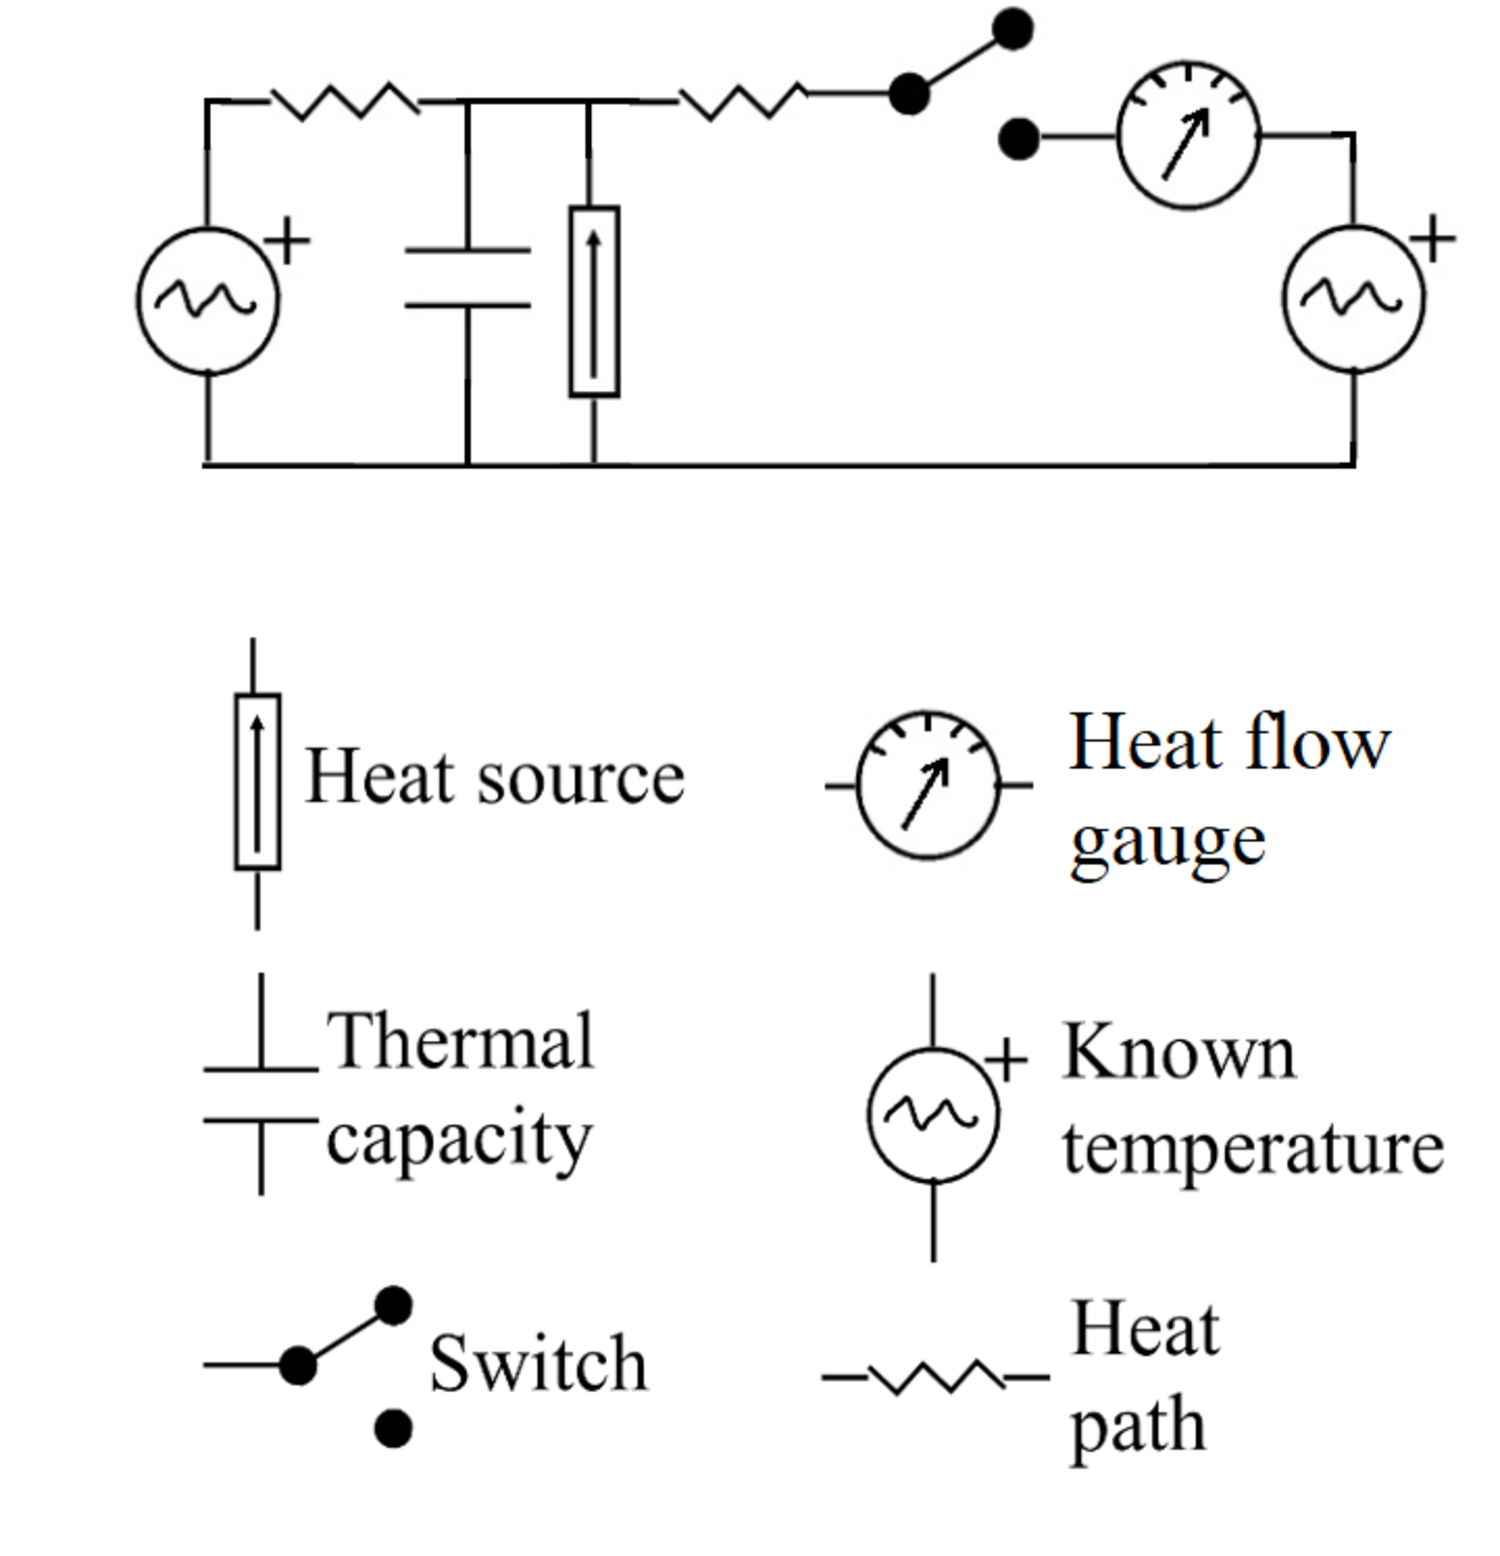
\includegraphics[width=4.5cm,height=4.5cm,keepaspectratio]{./pics/figAlf.pdf}}
\caption{Dual-mode RC network}\vspace*{-6pt}
  \label{fig:alf}
\end{figure}

The conditioning system is governed in our case by a thermostat with a timer that turns it on and off. For this reason one need to consider that the RC-network that represents the building needs to change topologies depending on the operation (on or off). We have considered a dual-mode RC-network as the one shown in Fig. \ref{fig:alf} and previously introduced by Ramallo-Gonz\'alez on \cite{ramalloidentifying}. 
These Grey-box models have been largely used in the past for building energy simulation. The reader is referred to \cite{bacher2011identifying}, \cite{coley1992second} and \cite{ramalloidentifying} for quantitative evidence of the accuracy of these kind of models.



\subsection{Black-box baseline models}

Our proposed black-box models are compared with two baseline approaches documented in literature. The first is a regression-based electricity load model and the second is a purely machine learning model that uses the inputs only at the same timestamp as the output.


\subsubsection{Time-of-week-and-temperature (TWT)}

This algorithm was introduced in \cite{mathieu2011quantifying}. We have chosen it because of its high accuracy, low complexity and low computational cost when compared with the results of other state-of-the-art methods used in a wide number of buildings \cite{granderson2016accuracy}. 

In this work the predicted load is the sum of two terms: a ``time of week effect" that allows each time of the week to have a different predicted load from the others, and a piecewise-continuous effect of temperature. 

The central point of this algorithm is the creation of several coefficients that will be estimated using multifple ordinary least square regression. There will be a coefficient for every ``time of the week". A time of the week is a unique instant of a week (Monday 1am, Monday 2am, and so on). For example, there will be $24 \times 5 = 120$ (24 hours and 5 working days) coefficients in the case of hourly predictions or  $4\times 24 \times 5 = 480$ in the case of 15 minutes prediction. In addition, some coefficients related to the temperature need also to be calculated. Basically, the range of outside temperature data is divided into 6 levels, each which has a coefficient assigned to it.

\subsubsection{Gaussian}

A Gaussian process (GP) modelling framework determining energy savings and uncertainty levels in measurement and verification (EM\&V) practice is presented in \cite{heo2012gaussian}.  In this work, the authors compare a black-box approach to the regular linear regression techniques that are widely explored in literature and state that GP models can capture both complex nonlinear and multivariable interactions and the multi-resolution trends of energy behavior thanks to the Bayesian approach under which they are developed. 

\subsection{Model Accuracy Metrics}

This work assesses model accuracy using two metrics: the mean absolute percentage of error (MAPE) and the coefficient of variation of the root mean squared error (CVRMSE).
The MAPE metric has been used in a wide number of electricity prediction studies \cite{fan2014development, edwards2012predicting}
. It expresses the average absolute error as a percentage and is calculated as it follows:

\[
 MAPE = \frac{1}{n}\sum_{i=1}^{n} |\frac{y_i-\bar{y_i}}{y_i}|\times 100,
\]

where $y_i$ is the real consumption, $\bar{y_i}$ is the predicted consumption and $n$ is the number of observations.

The CVRMSE has often been used in energy prediction studies \cite{quilumba2015using} and will also be used also here %26
. It evaluates how much error varies with respect
to the actual consumption mean and is calculated as follows:

\[
 CVRMSE = \frac{\sqrt{\frac{1}{n-1}\sum_{i=1}^{n}(y_i-\bar{y_i})^2}}{\bar{y}} \times 100,
\]


\subsection{Savings Metrics}

The IPMVP [13] and ASHRAE’s Guideline 14 [2] provide three methods with which to determine energy savings and uncertainty levels from energy efficiency measures. That which is most suitable for our approach is whole-building metering, since it compares the total energy demand or cost during pre-experiment and post-experiments periods.

%How to assess the accuracy and usefulness of whole-building energy models by testing predictions of baseline energy use against actual energy use being the objective to quantify and minimize the uncertainty in reported whole-building savings, which depends on baseline model effectiveness, building predictability, and depth of savings being measured \cite{kramer2013energy}.

The output of the predictive baseline models is the metered pre-experiment energy use energy$_{pre}$ which employs the environmental conditions as inputs for the model inputs$_{pre}$. The error in reported savings is proportional to the error in the baseline model forecasts.


\section{Use case}

The reference building in which the proposed procedure has been carried out in order to generate accurate building models is the Chemistry Faculty of the University of Murcia, which is a building used as a pilot for the H2020 ENTROPY project\footnote{http://entropy-project.eu/}.  

The data that is used in order to build and train our baseline corresponds to 1 year's worth of data, from February 2016 to February 2017. 

\begin{figure}[h]%\vspace*{4pt}
\centering
\centerline{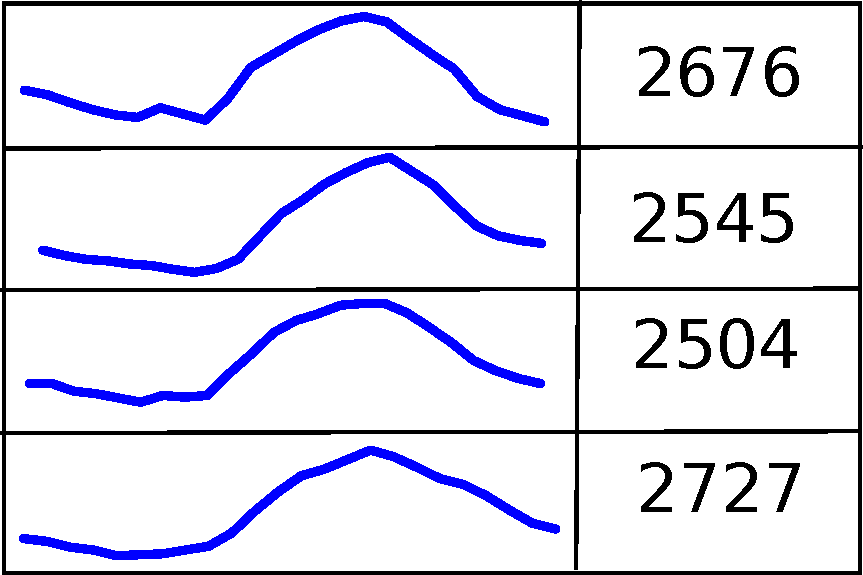
\includegraphics[width=4.5cm,height=4.5cm,keepaspectratio]{./pics/table_inputs_outputs.pdf}}
\caption{Daily temperature time series input and consumption output. Numbers in Watts hour}\vspace*{-6pt}
  \label{fig:inout}
\end{figure}

\subsection{Black-box approach}

Our black-box methodology is highly versatile with respect to the input data i.e.,  it allows the addition of variables with a minimal effort. We create the method in a constructive manner by relating the 24 temperature values of each day with the energy consumption of the building (see Fig. \ref{fig:inout}).

Having introduced the daily temperature time series, we considered that the addition of a categorical variable indicating the season was irrelevant. The subject building has several features that are typical of educational buildings: the load %is temperature-dependent load 
on weekends is substantially lower than that of weekdays and there are also differences among week days (mainly Fridays).
In these terms, we used analysis of variance (ANOVA) in order to determine whether there were differences between the consumption on the different days of the week (p-value = 0.001 $<$ 0.05). After carrying out a \textbf{post-hoc}  test we concluded that Fridays could be considered to behave differently to the other days of the week, which could be owing to lower occupation. Having attained this knowledge, we considered it necessary to add a dychotomus variable that indicates the kind of day of the week. Weekend and holiday consumption is estimated using the mean of previous weekends and holidays.

The algorithms that were found to be relevant for use within our black-box methodology are: Support Vector Regression (SVR), Regression Forest (RF) and Extreme Gradient Boosting (XGB). 

SVR works in a similar fashion to Support Vector Machines (SVM). Whereas SVM is a classification technique, SVR fits the optimal curve out of which the training data do not deviate more than a small number $\epsilon$. More specifically, during classification the samples that are close to the margin are penalized even if they are correctly classified, whereas in the regression method an acceptable deviation margin of the samples from the prediction curve is set.
The free hyperparameter of this model is C, the penalty parameter of the error term. C is the weight of how much the samples inside the margin contribute to the overall error.%, and ε, the distance between points predicted and the actual values.



Regression Forest is a type of ensemble learning method, in which a group of weak models combine to form a more powerful model. In Regression Forest, multiple regression trees are grown. In order to predict a new observation, each tree provides its own prediction after which the average of the output of each one is taken. The algorithm works by growing a tree from each random with replacement samples taken from the training. For each node, $m_{try}$ variables are selected at random out of the number of inputs. The best split in these $m_{try}$ is then used to split the node. The hyperparameter of Regression Forest that we will search for is the number of random variables that are taken into account in every split: $m_{try}$. 


XGB is built on the principles of gradient boosting and is designed for speed and performance (from which the term ``extreme" originates).
Gradient Boosted Regression is a technique that generates a prediction by means of an ensemble of weak prediction models that, in our case, are decision trees. The concept is to sequentially build the model by fitting a weak prediction model on the weighted training data set, in which the higher weights are assigned to samples that were previously difficult to predict.

The free hyperparameters that are adjusted in this model are the maximum depth limit of the number of nodes in the tree, the minimum number of samples required to split an internal node and the learning rate by which the contribution of each tree is shrunk.

For the sake of comparison, we also employ the Gaussian Process to model the instantaneous consumption prediction using the current input values (mean daily temperature for daily consumption or mean hourly temperature for hourly consumption).


\subsection{Grey-box approach}

In the case of our grey-box methodology, a topology was selected that could adequately represent the building.


Once the system had been defined, an optimization algorithm was used to find the values that minimize the RMSE (10 minutes intervals) of the simulated power consumption. To ensure that the data was used appropriately, the total electricity consumption was separated onto an un-seasonal component and a seasonal one. The un-seasonal component was used as electric loads and the seasonal component was considered to be the heating and cooling load. The building is equipped with a boiler and radiators network that contribute to some of the heating loads. In order to take into account this effect, the prelimiary estimation was made using the summer period. From which the portion of heating provided by radiators was extracted. This ratio was used in the consecutive calculations.

The optimization method employed to find the parameters of the model was the simplex method. The termination criterion was to attain a change in the solution that was smaller than 0.01 in all the parameters. %The calculation took approximately 6 minutes on a i5 Intel computer 2.7 running single threaded.


\subsection{Results}

The prediction metrics are summarized on Table I. The first three methods: SVR, RF, XGB  belong to the group of black-box models and are blind to the physics of the problem. We also have the TWT, the GP and the Grey-box model, the last of which contains information regarding the physical phenomenon of the model topology. As can be seen, they return the best results when compared to the Gaussian method, that is applied in a more traditional manner, i.e., by relating the instantaneous consumption measurement with the instantaneous inputs measurements and also with our grey-box model approach. 

Of the three black-box methods, Random Forest is that which stands out since it attained a CVRMSE of 9 and 5 \%  and a MAPE of 6, and 4.5 \% for the daily and weekly predictions respectively. We have plotted the predicted vs the real daily consumption (measured in Watt-hour) in Fig. \ref{fig:daily} and the weekly consumption in Fig. \ref{fig:weekly} .

\begin{center}
\captionof{table}{Metrics}
\resizebox{\columnwidth}{!}{%
\begin{tabular}{cc|c|c|c|c|c|c|c}
\cline{3-8}
& & \multicolumn{6}{ c| }{Models} \\ \cline{3-8}
& & SVR & \textbf{RF} & XGB & TWT & Gauss & Grey   \\ \cline{1-8}
\multicolumn{1}{ |c  }{\multirow{2}{*}{Daily} } &
\multicolumn{1}{ |c| }{CVRMSE} & 12.4 & \textbf{9} & 11& 14.9  & 17.45 & 33.57      \\ \cline{2-8}
\multicolumn{1}{ |c  }{}                        &
\multicolumn{1}{ |c| }{MAPE} & 7.2 & \textbf{6} & 7.3& 12.3 & 15.01 & 43.02      \\ \cline{1-8}
\multicolumn{1}{ |c  }{\multirow{2}{*}{Weekly} } &
\multicolumn{1}{ |c| }{CVRMSE} & 6.4 & \textbf{5} & 6.2 & 11.1 & 16.3 & 19.53  \\ \cline{2-8}
\multicolumn{1}{ |c  }{}                        &
\multicolumn{1}{ |c| }{MAPE} & 5.2 & \textbf{4.5} & 5.5 & 9.4 & 12.3 & 15.48  \\ \cline{1-8}
\end{tabular}
}
\end{center}




%\begin{figure}[h]%\vspace*{4pt}
%\centering
%\centerline{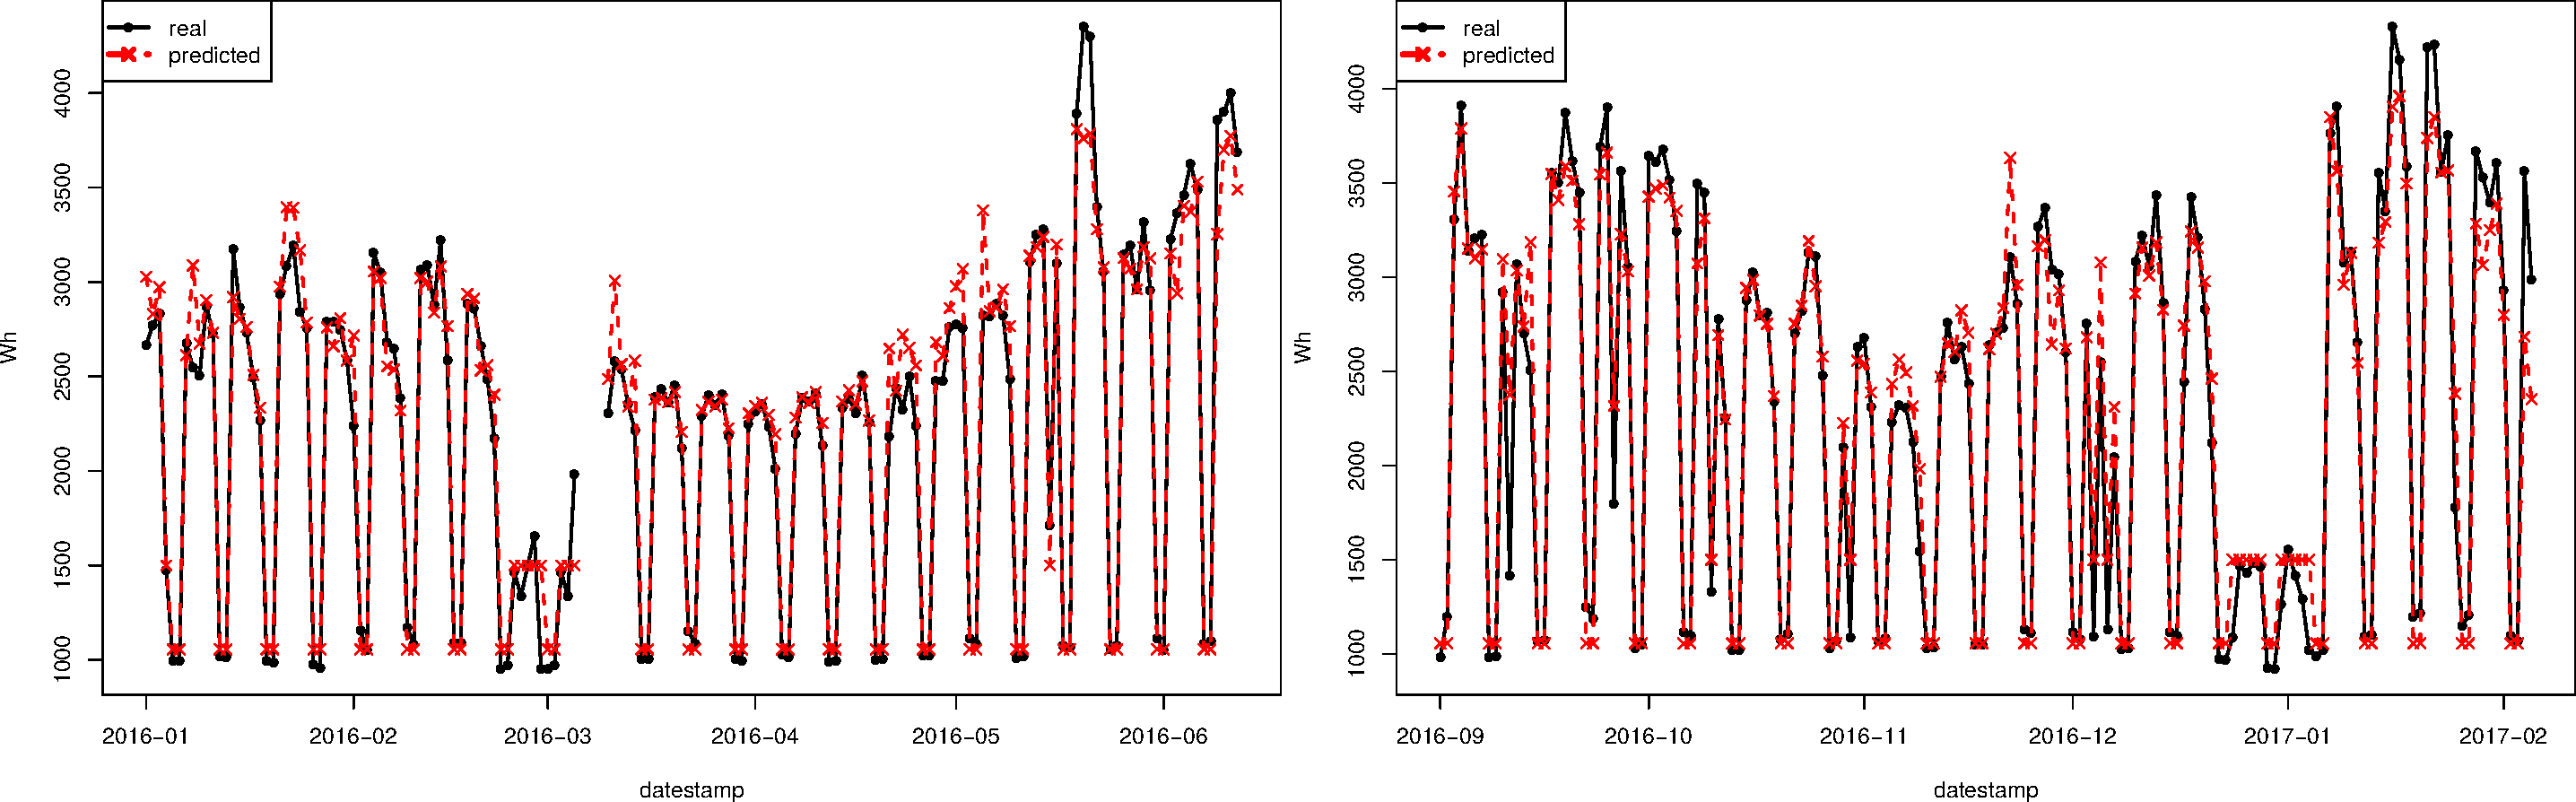
\includegraphics[width=15.5cm,height=15.5cm,keepaspectratio]{./pics/two_daily.pdf}}
%\caption{Daily predictions using RF and real consumption}\vspace*{-6pt}
%  \label{fig:daily}f
%\end{figure}

\begin{figure*}[t!]
  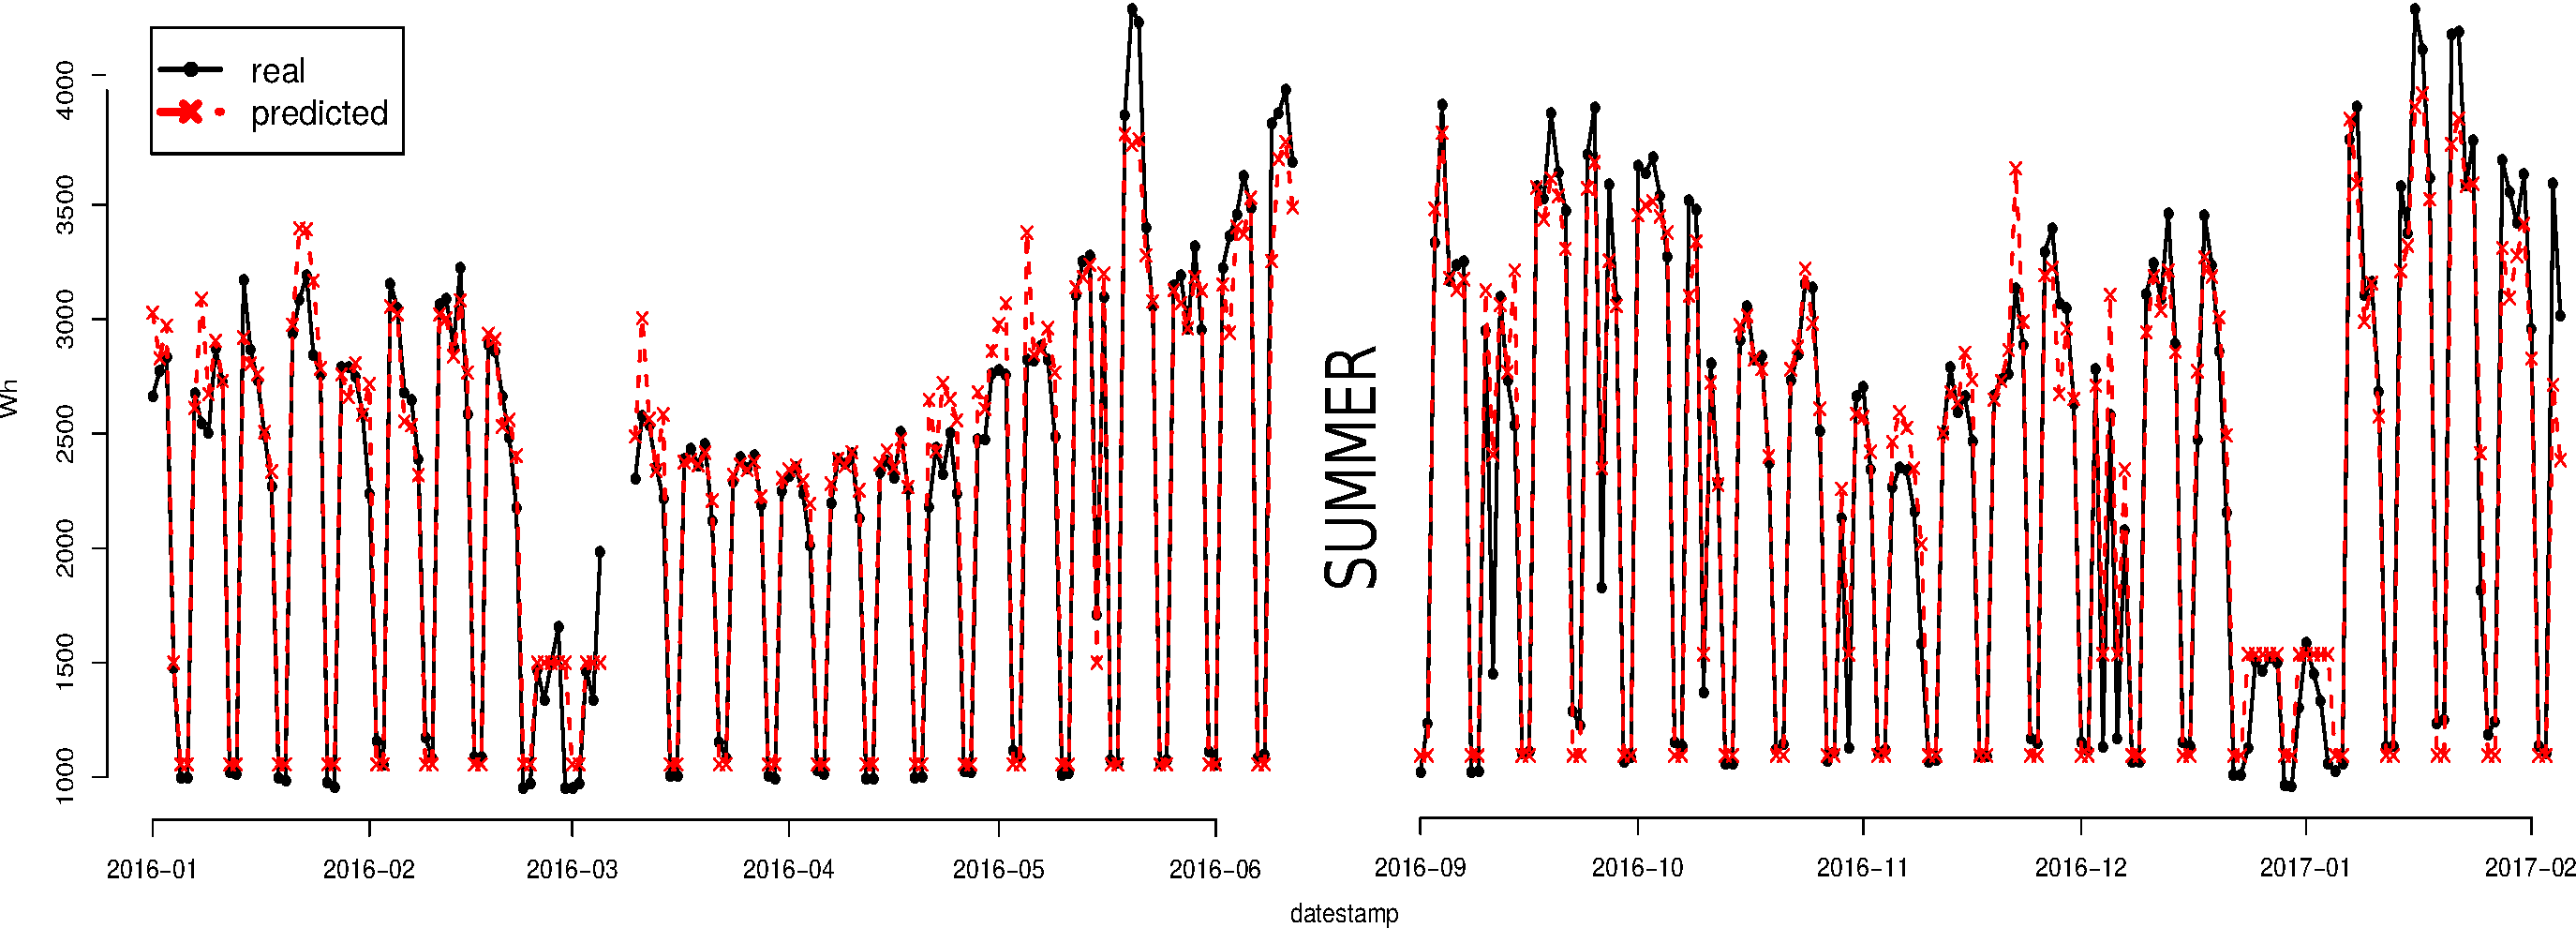
\includegraphics[width=17cm,height=17cm,keepaspectratio]{./pics/two_daily-iii.pdf}
  \caption{Daily predictions using RF and real consumption}
  \label{fig:daily}
\end{figure*}

%\begin{figure}
%\centering
%\begin{subfigure}[b]{0.55\textwidth}
%   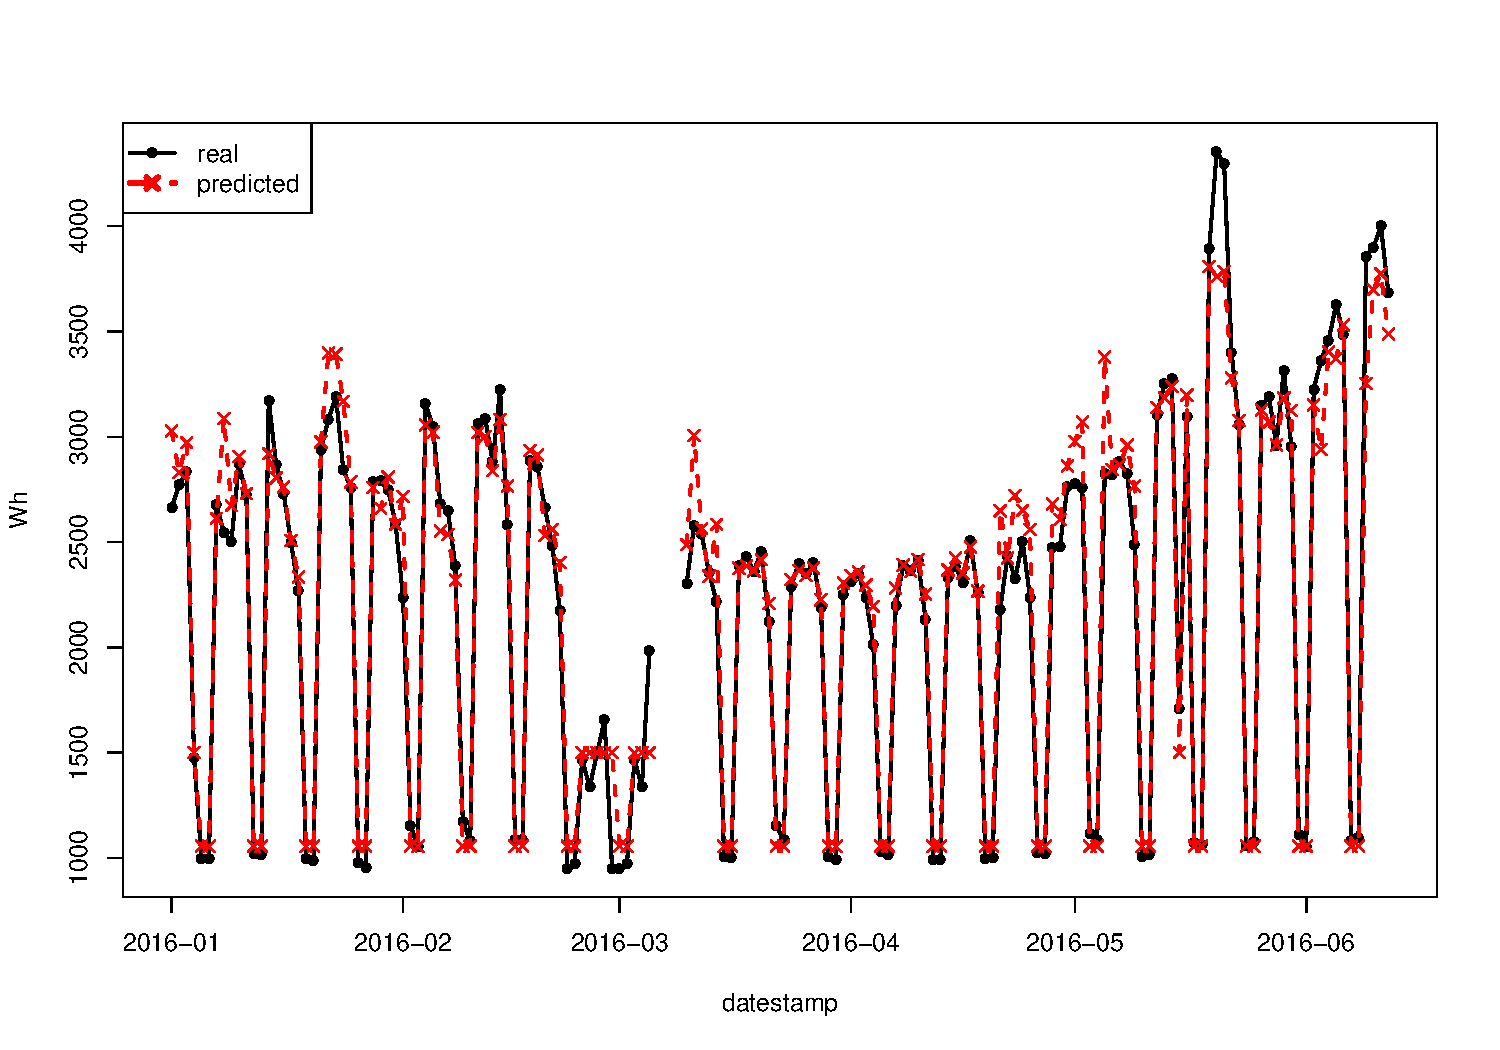
\includegraphics[width=8cm,height=5cm]{./pics/daily_RF1.pdf}
%   \caption{}
%   \label{fig:Ng1} 
%\end{subfigure}
%
%\begin{subfigure}[b]{0.55\textwidth}
%   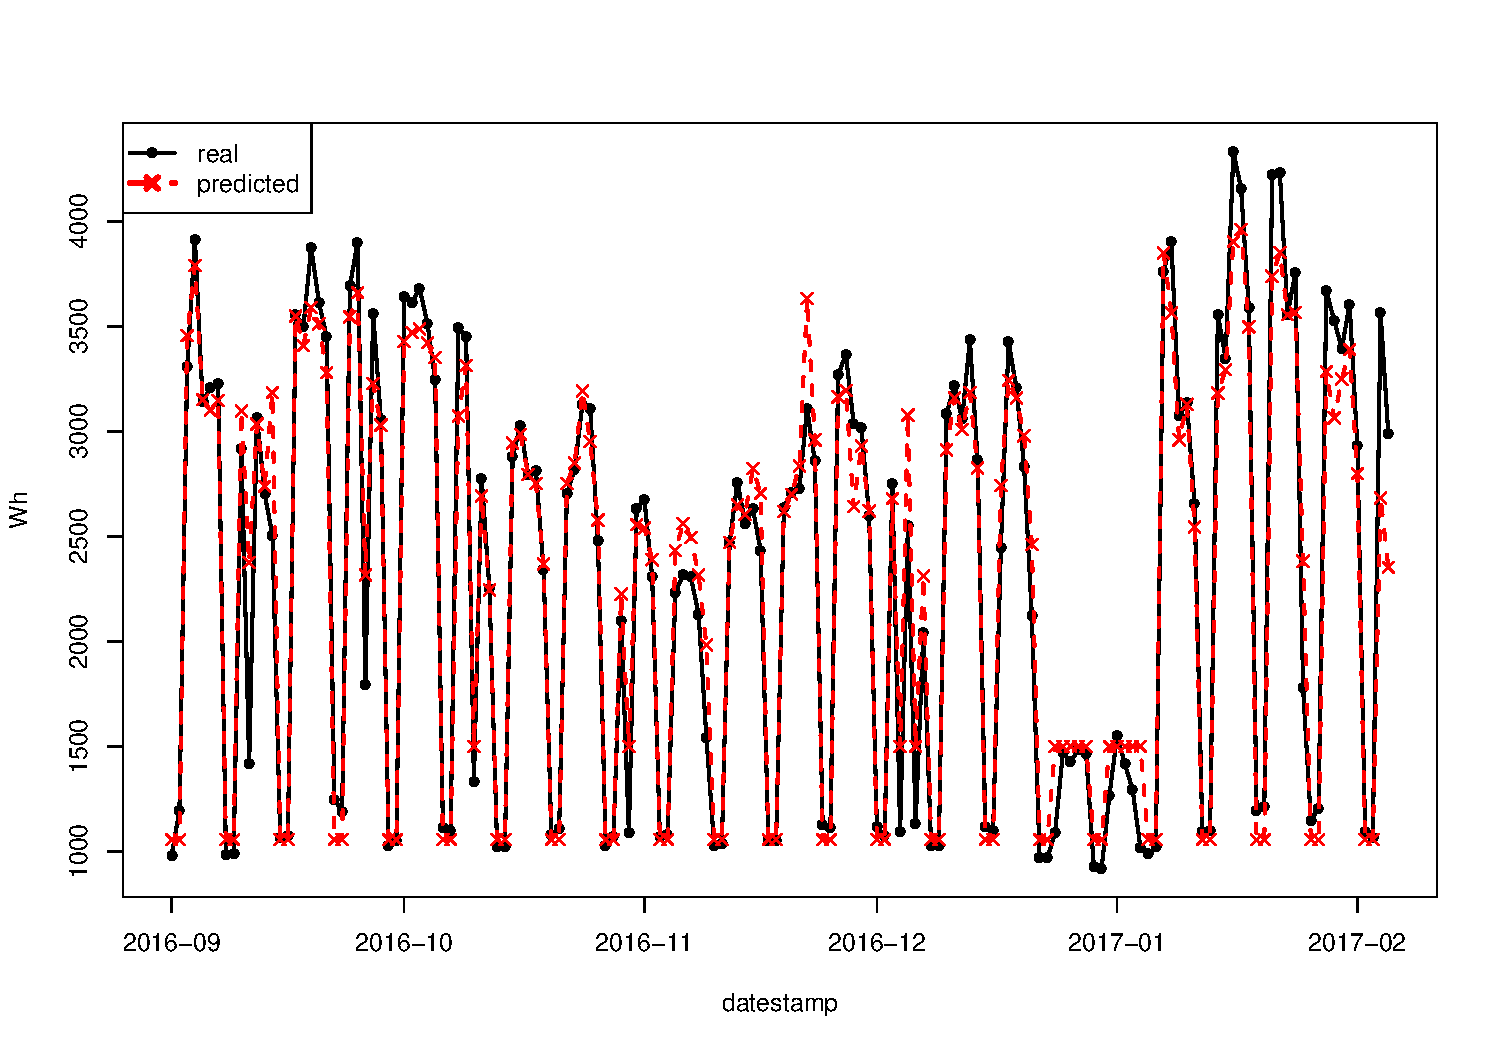
\includegraphics[width=8cm,height=5cm]{./pics/daily_RF2.pdf}
%   \caption{}
%   \label{fig:Ng2}
%\end{subfigure}
%\label{fig:daily}
%\caption[Two numerical solutions]{(a) (b) As for (a) but over a second period of time}
%\end{figure}

\begin{figure*}[t!]\label{fig:weekly}%\vspace*{4pt}
\centering
\centerline{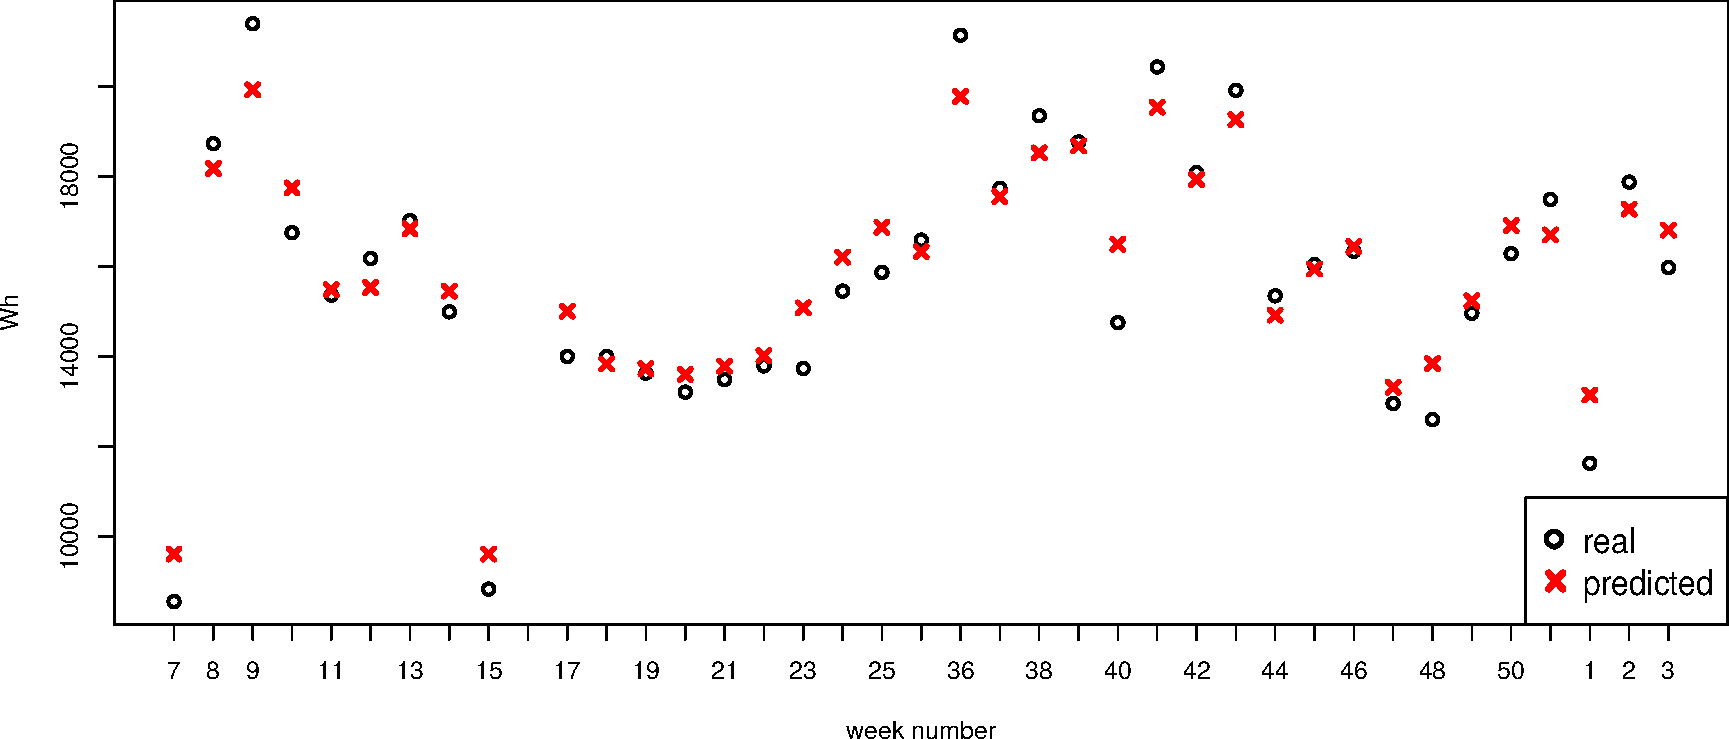
\includegraphics[width=12cm,height=12cm,keepaspectratio]{./pics/weekly.pdf}}
\caption{Weekly predictions using RF and real consumption}\vspace*{-6pt}
  \label{fig:weekly}
\end{figure*}

\section{Discussion}

As mentioned previously, the objective of this paper is to evaluate whether the fact that the RC-networks in the grey-box inverse modeling contain basic information converning the physical system (i.e. what the thermodynamics of the building should be like) have any advantages for the prediction of energy consumption for a smart building with measurement and verification purposes. They were, therefore, compared to our proposed state-of-the-art black-box method in which no prior high level information about the system is included (i.e. the models are blind to the physics of the problem) and which combines statistical analysis and machine learning techniques. %For that, the errors and computational times of a grey-box model have been estimated for the case under study.

%This work has introduced two ways for predicting energy consumption for use in applications focused on whole-building measurement and verification for energy efficiency programs.

%One way is purely data-driven, based on statistical analysis and machine learning algoritms, the so called black-box approach. The other way is based on the physical properties of the building and its relationship with the data, that is a grey-box approach.

We have shown that by using the daily temperature time series we are able to capture the people's behaviour better than if instantaneous values are used to predict consumption (Gaussian) or if we use a barrage of coefficients in linear regression to model each small part of the day (TWT). 

This result could, in some respects, have been anticipated, since energy consumption is greatly dominated by human behavior. The physics of the building can capture the response of passive elements such as walls and windows, but behavioral patterns are out of their scope.

One drawback of baseline data-driven models is that they ignore the correlation between timestamps. TWT creates artificial features in order to model each moment independently. We understand that the input data are time series and we indirectly consider all the interactions that the building and temperature have as regards consumption.
Moreover, the application of regression techniques has to be preceded by the assessment of the assumptions that have to be fulfilled: normality, little multi-collinearity, no auto correlation and homocedasticity. However, black-box models do not require such assumptions.


We have, therefore, created a methodology with which the combination of time series and current state variables is possible and that provides a wide variety of techniques related to time series that can be used to improve the results of the analysis.

\section{Conclusions and future work}

After applying all the baseline models, grey-box approach and black-box approach, we have seen that black-box models outperform the rest.

%A very important characteristic of the black-box approach is its generality. Even if we would have obtained similar results with the grey-box models, black-box models are clearly more generalizable than the previous. 


One future avenue of research consists of applying the same models to several buildings that share some characteristics. That is, they belong to the same environment: different faculties of a university (where students and professors behave similarly in all the buildings), several houses of a neighborhood or different commercial buildings in the same city.

Reducing the total time required for EM\&V is the key to scaling the deployment of energy efficiency projects in general, and reducing overall costs \cite{granderson2015automated}. It is for this reason that a transfer learning approach should be considered in future studies in order to reduce the quantity of data that needs to be collected to create a reasonable building model.

Moreover, a broader study on the means employed to introduce the time series into the algorithms should be carried out. This implies applying time series segmentation and representation techniques in order to discover more representative means of introducing the data, or also considering feature selection techniques.


Overall, we believe that the work reported in this paper has explored yet another discipline in which data-driven methods are outperforming traditional methods based on physics. The results once more demonstrate that data science can provide answers that are “as good as” or “better than” physically informed approaches.

\section*{Acknowledgements}

This work has been partially funded by MINECO TIN2014-52099-R project (grant BES-2015-071956) and ERDF funds, by the European Commission through the H2020-ENTROPY-649849 EU Project. Ramallo-Gonz\'alez would like to thank CARM via Fundaci\'on S\'eneca for the program Saavedra Fajardo, project number: 20035/SF/16.


% An example of a floating figure using the graphicx package.
% Note that \label must occur AFTER (or within) \caption.
% For figures, \caption should occur after the \includegraphics.
% Note that IEEEtran v1.7 and later has special internal code that
% is designed to preserve the operation of \label within \caption
% even when the captionsoff option is in effect. However, because
% of issues like this, it may be the safest practice to put all your
% \label just after \caption rather than within \caption{}.
%
% Reminder: the "draftcls" or "draftclsnofoot", not "draft", class
% option should be used if it is desired that the figures are to be
% displayed while in draft mode.
%
%\begin{figure}[!t]
%\centering
%\includegraphics[width=2.5in]{myfigure}
% where an .eps filename suffix will be assumed under latex, 
% and a .pdf suffix will be assumed for pdflatex; or what has been declared
% via \DeclareGraphicsExtensions.
%\caption{Simulation Results}
%\label{fig_sim}
%\end{figure}

% Note that IEEE typically puts floats only at the top, even when this
% results in a large percentage of a column being occupied by floats.


% An example of a double column floating figure using two subfigures.
% (The subfig.sty package must be loaded for this to work.)
% The subfigure \label commands are set within each subfloat command, the
% \label for the overall figure must come after \caption.
% \hfil must be used as a separator to get equal spacing.
% The subfigure.sty package works much the same way, except \subfigure is
% used instead of \subfloat.
%
%\begin{figure*}[!t]
%\centerline{\subfloat[Case I]\includegraphics[width=2.5in]{subfigcase1}%
%\label{fig_first_case}}
%\hfil
%\subfloat[Case II]{\includegraphics[width=2.5in]{subfigcase2}%
%\label{fig_second_case}}}
%\caption{Simulation results}
%\label{fig_sim}
%\end{figure*}
%
% Note that often IEEE papers with subfigures do not employ subfigure
% captions (using the optional argument to \subfloat), but instead will
% reference/describe all of them (a), (b), etc., within the main caption.


% An example of a floating table. Note that, for IEEE style tables, the 
% \caption command should come BEFORE the table. Table text will default to
% \footnotesize as IEEE normally uses this smaller font for tables.
% The \label must come after \caption as always.
%
%\begin{table}[!t]
%% increase table row spacing, adjust to taste
%\renewcommand{\arraystretch}{1.3}
% if using array.sty, it might be a good idea to tweak the value of
% \extrarowheight as needed to properly center the text within the cells
%\caption{An Example of a Table}
%\label{table_example}
%\centering
%% Some packages, such as MDW tools, offer better commands for making tables
%% than the plain LaTeX2e tabular which is used here.
%\begin{tabular}{|c||c|}
%\hline
%One & Two\\
%\hline
%Three & Four\\
%\hline
%\end{tabular}
%\end{table}


% Note that IEEE does not put floats in the very first column - or typically
% anywhere on the first page for that matter. Also, in-text middle ("here")
% positioning is not used. Most IEEE journals/conferences use top floats
% exclusively. Note that, LaTeX2e, unlike IEEE journals/conferences, places
% footnotes above bottom floats. This can be corrected via the \fnbelowfloat
% command of the stfloats package.



% trigger a \newpage just before the given reference
% number - used to balance the columns on the last page
% adjust value as needed - may need to be readjusted if
% the document is modified later
%\IEEEtriggeratref{8}
% The "triggered" command can be changed if desired:
%\IEEEtriggercmd{\enlargethispage{-5in}}

% references section

% can use a bibliography generated by BibTeX as a .bbl file
% BibTeX documentation can be easily obtained at:
% http://www.ctan.org/tex-archive/biblio/bibtex/contrib/doc/
% The IEEEtran BibTeX style support page is at:
% http://www.michaelshell.org/tex/ieeetran/bibtex/
\bibliographystyle{IEEEtran}
% argument is your BibTeX string definitions and bibliography database(s)
\bibliography{IEEEabrv,bib.bib}
%
% <OR> manually copy in the resultant .bbl file
% set second argument of \begin to the number of references
% (used to reserve space for the reference number labels box)
%\begin{thebibliography}{1}

%

%\end{thebibliography}




% that's all folks
\end{document}


